%***************************************************
% body

\section{Introduction}
Plasma-based accelerators are capable of producing accelerating fields that are orders of magnitude larger than the fields generated in conventional RF cavities. Two-bunch plasma wakefield acceleration (PWFA) is a method that utilizes these fields to accelerate mono-energetic beams of electrons. In two-bunch PWFA, the leading ``drive" bunch creates a wake in a cold, neutral plasma. The trailing ``witness" bunch follows the drive bunch by roughly half the plasma wavelength at an accelerating phase of the wake. This scheme is challenging because the wavelength associated with high-gradient plasma wakes is small. Typical experiments at FACET utilize plasma wakefields with wavelengths from 100-200 $\mu$m. By contrast, the wavelength of SLAC's s-band cavities is roughly 10.5 cm. Conventional bunch compression techniques preclude the possibility of the using electron bunches in consecutive RF buckets for PWFA at FACET.

We have developed a technique called notch-collimation to create two bunches from a single electron bunch. Our technique takes advantage of the linear head-tail energy correlation, or chirp, in the beam distribution. The FACET beam is chirped as part of the three stage bunch compression scheme that shrinks the beam from an initial bunch length of 6.6 mm to a final bunch length that can be as short as 20 $\mu$m. In the final stage of compression, a tantalum blade is inserted into the beamline at a point of high dispersion. The blade cuts out a portion of the beam's energy spectrum, which as a result of the chirp corresponds to a longitudinal chunk of the bunch profile. The final bunch profile is a high-contrast double gaussian, or two-bunch structure.

The notch-collimation procedure is sensitive to small variations in the beam's longitudinal phase space at the entrance of the final bunch compressor. In order to verify that we are creating the correct final bunch distribution, we use an x-band transverse deflecting cavity (TCAV) to streak the beam and image the longitudinal profile. In addition, we have developed a novel tomographic method for reconstructing the longitudinal phase space of the beam. These diagnostics are critical for beam tuning and understanding experimental results.

\section{Longitudinal Phase Space Evolution}
The electron beam at FACET is generated from a thermionic cathode and quickly accelerated to 1.19 GeV before being transported to the North Damping Ring (NDR), shown on the left side of Figure~\ref{schem}. The bunch radiatively damps to an equilibrium bunch length and an equilibrium energy spread during the course the 16 ms store. The bunch length was measured to be $\sigma_z = 6.6$ mm with a streak camera. Figure~\ref{streak} shows the synchrotron radiation generated by the beam in one of the bends in the ring as imaged by the streak camera. The equilibrium energy spread is solely a function of the beam energy and lattice parameters and it is calculated to be $\sigma_{\delta} = 7.0 \times 10^{-4}$. There is no time-energy correlation of the beam in the ring, so the initial longitudinal phase space is given by $\varepsilon_{z0} = \sigma_z \sigma_{\delta} = 5$ MeV$\cdot$mm. 

\begin{figure*}[t]
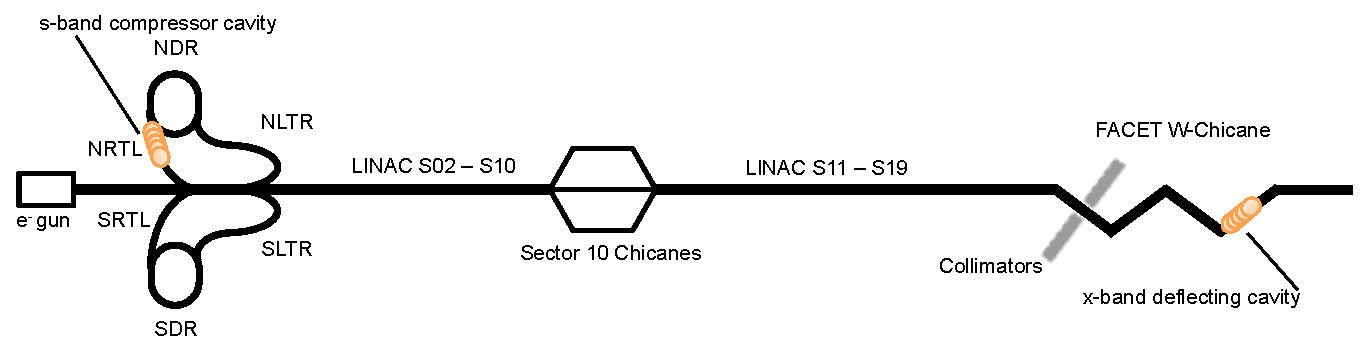
\includegraphics[width=\textwidth,height=4cm]{figures/facet_schem.pdf}
  \caption{Overview of the FACET Linac.}
  \label{schem}
\end{figure*}

\begin{figure}[hb]
  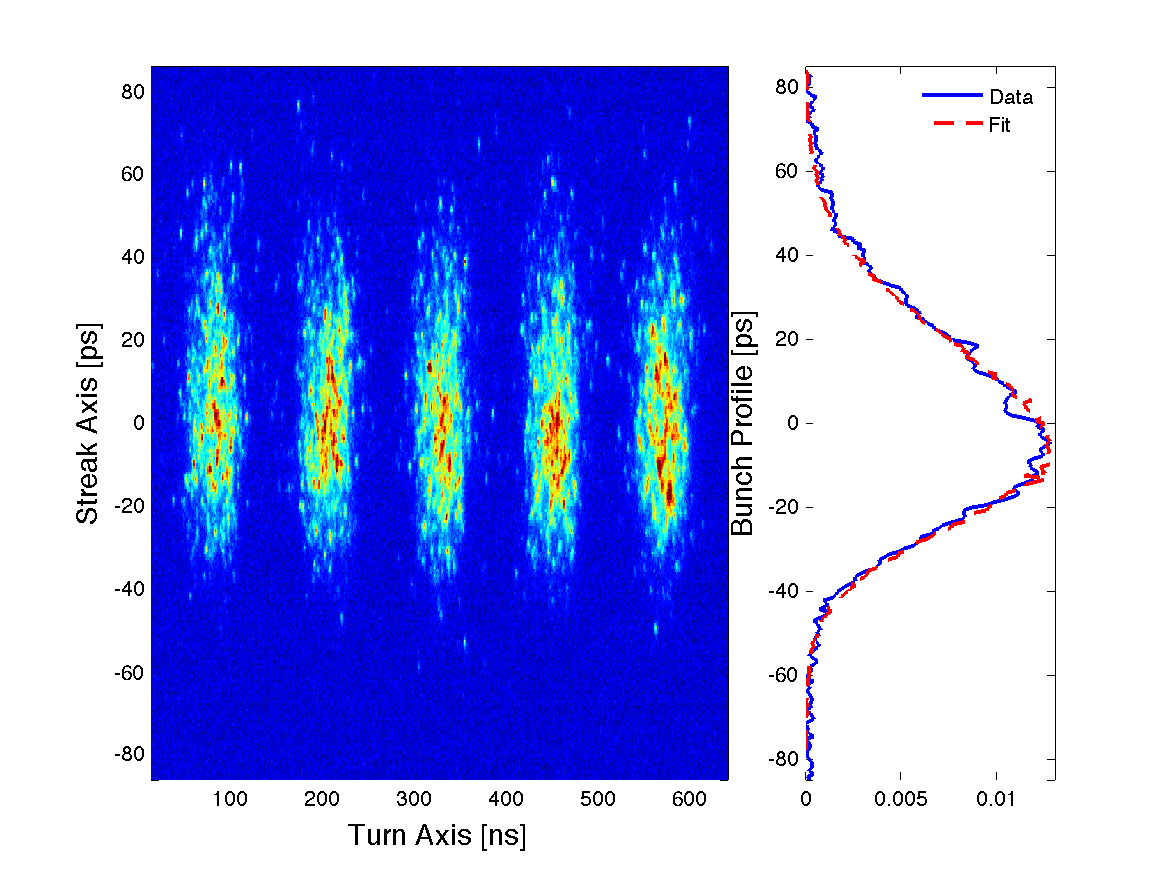
\includegraphics[width=\columnwidth]{figures/combo.pdf}
  \caption{Streak camera image of the final five turns before extraction from NDR. The bunch profile on the right is the average of the five turns shown, fit to an asymmetric gaussian with $\sigma_t = 22$ ps and asymmetry parameter -0.2.}
  \label{streak}
\end{figure}

Upon extraction from the NDR, the beam is chirped an the s-band compressor cavity. The beam is compressed by a factor of 10 in the North Ring to Linac (NRTL) chicane and enters the Linac with a 600 $\mu$m RMS bunch length. The bunch is slightly over-compressed, with a residual low-to-high chirp, so as to minimize the impact of wakefields in the linac. The bunch is accelerated in the first kilometer of the linac with a net phase of -20 degrees with respect to the crest (in SLAC coordinates, negative angles are ahead of crest). FACET uses a unique chirping scheme that staggers the phasing of the beam over nine linac sectors. The staggered chirp process is depicted in Figure~\ref{stag}. By accelerating on crest or nearly on crest in the first few sectors, the beam becomes stiff and more resistant to emittance dilution from transverse wakefields. The later sectors have stronger phasing, up to -55 degrees off crest, in order to achieve an average of -20 degrees chirp prior to the Sector 10 Chicane. While this scheme has the advantage of reducing emittance growth, it makes the beam more sensitive to phase errors in the highly chirped sectors.

\begin{figure}[hb]
  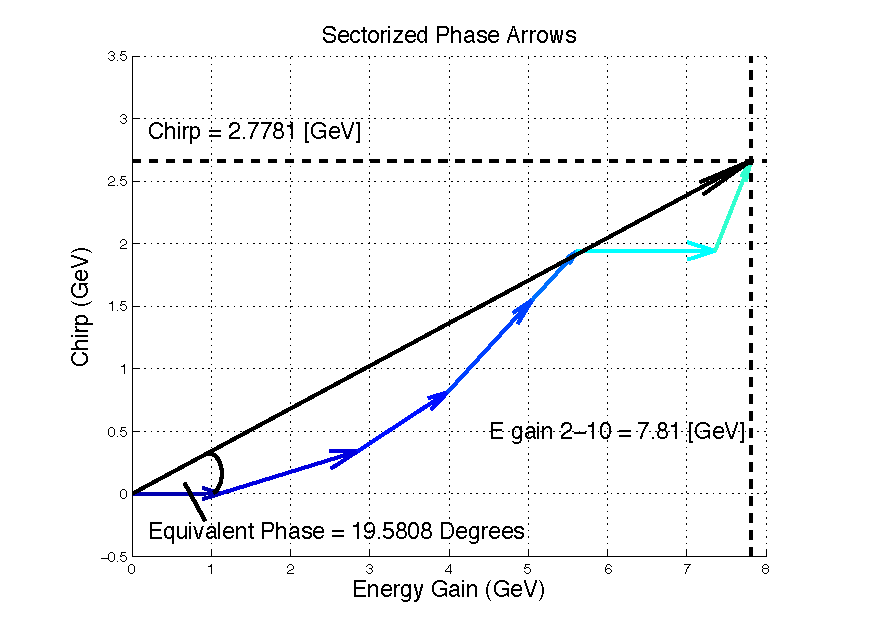
\includegraphics[width=\columnwidth]{figures/stag.pdf}
  \caption{Diagram showing the phasing in sectors 2-10 at FACET. Each arrow represents the phase and amplitude of the accelerating sector. Note that the chirping angle is depicted as a positive value for clarity.}
  \label{stag}
\end{figure}

The bunch is compressed by another factor of 10 in the Sector 10 Chicane. Again, the bunch is over-compressed, this time with a residual high-to-low chirp. The very short (50 $\mu$m), very high charge (3.2 nC) bunch drives a high-amplitude longitudinal wakefield in the SLAC s-band cavities. The wakeloss function $W(z)$ is a convolution of the cavity wake structure and the bunch profile, but for very short bunches it is roughly linear over the core of the bunch. The net effect of the wakefields in the second kilometer of the linac is to provide a mostly linear high-to-low chirp that will be leveraged for bunch compression in the FACET W-Chicane. Figure~\ref{sect19} shows a LiTrack simulation of the longitudinal phase space prior to final compression in the W-Chicane.

\begin{figure}[hbt]
  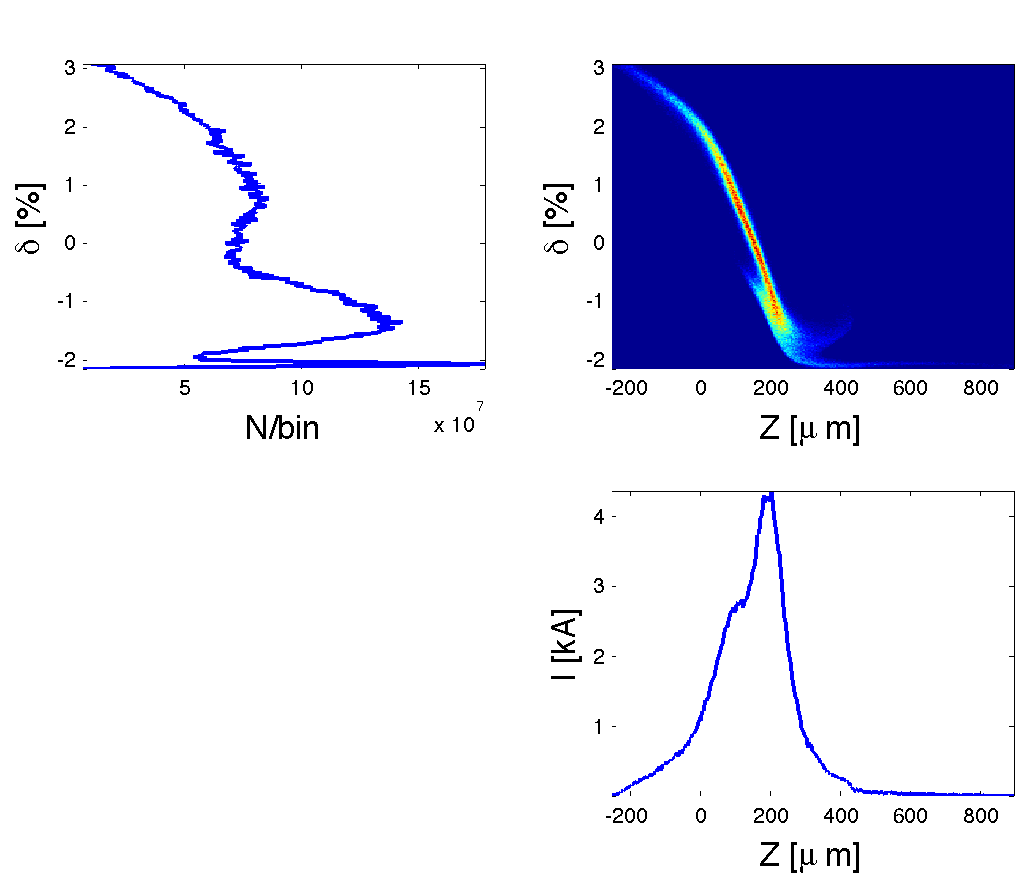
\includegraphics[width=\columnwidth]{figures/sect19.pdf}
  \caption{LiTrack simulation of the longitudinal phase space at the entrance of the FACET W-Chicane modeled with design parameters. The beam travels to the left.}
  \label{sect19}
\end{figure}

The FACET W-Chicane is a unique lattice that features adjustable $R_{56}$.  When extremely short bunches are needed, the chicane is tuned to $R_{56} = 5$ mm and yields a gaussian bunch with $\sigma_z = 20~\mu$m. For the two-bunch setup, the $R_{56} = 10$ mm, which over-compresses the bunch with a residual low-to-high chirp. In this case, the uncollimated bunch is non-gaussian with an RMS of 100-200 $\mu$m. A thin tantalum blade, referred to as the notch collimator, is inserted into the beam at a point where the ratio $\eta \delta / \sqrt{ \beta \varepsilon}$ is maximized early in the chicane. The notch collimator removes charge from the core of the energy spectrum, which corresponds to center of the bunch profile as a result of the $z-\delta$ correlation. Jaw collimators are used to remove high and low energy tails that lack $z-\delta$ correlation. This improves the final contrast of the two-bunch longitudinal profile.

\begin{figure}[hbt]
  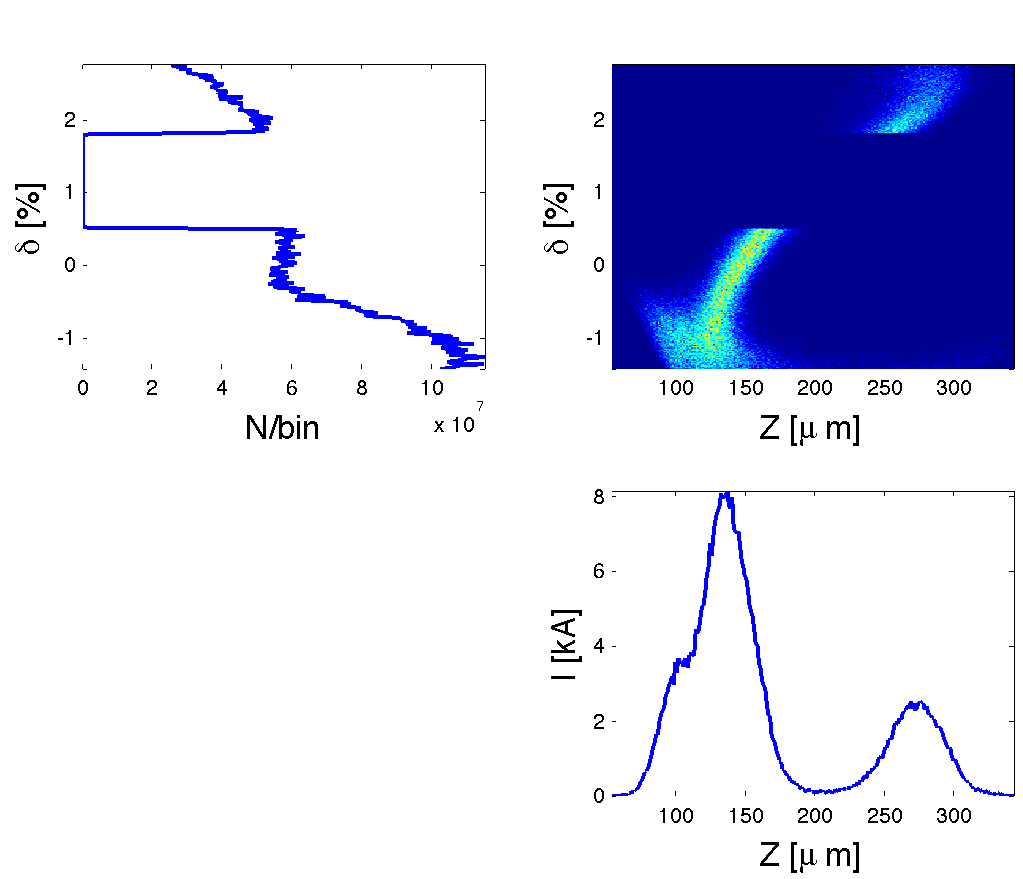
\includegraphics[width=\columnwidth]{figures/sect20.pdf}
  \caption{LiTrack simulation of the longitudinal phase space after collimation and compression in the W-Chicane.}
  \label{sect20}
\end{figure}

\section{Longitudinal Phase Space Diagnostics}
A transverse deflecting x-band cavity (TCAV) is located near the end of the chicane, close to maxima in $\beta_y$. The TCAV is used as a vertical streaking device; electrons with different longitudinal positions $z$ in a bunch experience different transverse deflecting fields. The particles are displaced vertically according to
\begin{equation}
\Delta Y = R_{34}\frac{e V_{rf}}{E_0}\sin{kz}
\end{equation}
and $R_{34}$ is the matrix element between the TCAV and the location where the streaked beam is imaged on a screen. The TCAV phase is calibrated such that the position $z=0$ in the beam corresponds to the zero crossing of the deflecting wave. The TCAV is the only diagnostic that has been used experimentally to resolve femtosecond beam structures. However, the TCAV is a destructive diagnostic, so it is not used while taking experimental data with plasma.

A half-period wiggler magnet is located just downstream of the TCAV at a dispersive point with the same $\eta$ and $\beta$ as the notch collimator. The wiggler deflects the horizontally-dispersed beam vertically. This generates a streak of synchrotron x-rays which are intercepted by a scintillating YAG:Ce crystal millimeters above the beam path. The x-ray streak encodes the energy spectrum of the beam onto the crystal, which is imaged by a CCD camera. On average, each 20.35 GeV electron radiates away 67 KeV of x-rays Emittance dilution due to ISR and CSR is negligible, so we the wiggler/YAG energy spectrometer is non-destructive. This is a particularly useful diagnostic, because it provides information about the longitudinal phase space on every shot.

\section{Longitudinal Phase Space Tomography}
We have developed a novel diagnostic technique that allows us to reconstruct the beam's longitudinal phase space. We use the notch and jaw collimators to create a narrow momentum aperture, or slit, which we scan across the path of the dispersed beam. A fraction of the beam is transmitted through the slit and is streaked at the TCAV. Bunch profiles are measured for each setting of the momentum slit. Figure~\ref{raw_data} shows the raw data from the measurement.

\begin{figure}[hbt]
  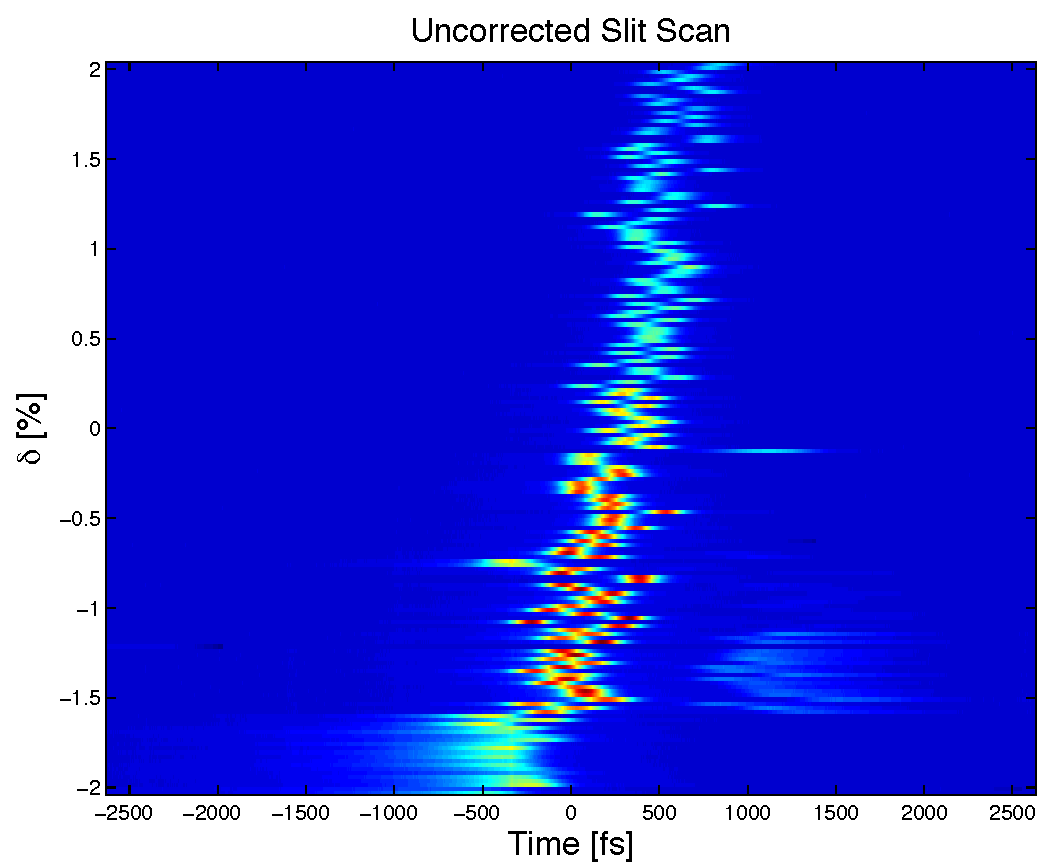
\includegraphics[width=\columnwidth]{figures/uncor.pdf}
  \caption{Raw data from the tomographic slit scan measurement.}
  \label{raw_data}
\end{figure}

The raw data has to be corrected for two effects. First, there is an inherent arrival time jitter of the beam relative to the RF phase of the TCAV with an RMS of roughly 250 fs. Second, there is a drift of the cavity phase relative to the beam caused by the heating of the cavity. The drift can be measured by 

\section{Conclusion}
Fuck this I am out.